\documentclass[11pt,twoside,a4paper]{report}
\usepackage{appendix}
\usepackage{geometry}
\usepackage{graphicx}
\usepackage{pdfpages}

% set the default, standard, geometry
\geometry{left=25mm, right=25mm, top=25mm, bottom=25mm}

\setlength{\parskip}{\baselineskip}
\clubpenalty10000
\hyphenpenalty10000
\widowpenalty10000

\begin{document}

\title{ID2216 Developing Mobile Applications\\Assignment 4 Report}
\author{Rafael Aldana (rafaelap@kth.se)\\Vincent Delitz (delitz@kth.se)\\Ruth Eriksson (ruthe@kth.se)}
\date{\today}
\maketitle



\tableofcontents
\thispagestyle{empty}

%\listoffigures

%\listoftables

\renewcommand{\chaptername}{Assignment}
\setcounter{chapter}{3}


\chapter{App web service}
\label{assignment:app-web-service}

\section{Overview}

After we received first feedback from testers for our initial draft of the Android app, we aimed to make it more useful and handy by integrating some web services. We decided to use therefore the Google Maps API, Facebook API, and SQLite relational database management system.

\begin{itemize}

\item The Facebook API was used in order to let users register with their Facebook account in our app, so that they do not need an extra account for our app. Furthermore, the Facebook API enables us to integrate in the future more and better customized services for the user.

\item In order to display the location of the pick-up place in a more convenient way, we made use of Google Maps API, so that the user can see where on the map the pick-up place is located.

\item To store our data in a manageable and clear manner, we use SQLite which is a database API optimized for Android applications.

\end{itemize}

\section{Development}

The great benefit from the Facebook API login functionality is that users are generally already logged into their Facebook account on their smartphones. Thus, a single button click in our application is sufficient to authenticate the user and give him access to the new offer screen. This reduces the effort for the user significantly and furthermore, he will stay logged in for the future, unless he does not explicitly log out.

To develop this feature, we had to register ourselves at the Facebook developer page first and our app then. Therefore, we needed to create a dedicated app hash key that is used by Facebook to identify our application. Then, if the user logs himself in to the app, we will receive an access token with which we can retrieve information from the user's profile, such as the name, email address, or profile picture in a JSON object. We made use of this information and displayed it in the navigation drawer menu in our MainActivity.

For the display of the pick-up place of SL cards, we made use of the Google Maps API. Luckily, Android Studio offers the possibility to create a Google Maps activity right away by default. That is why we only needed to adapt this activity according to our needs and moreover, register our application at the Google developers web page. 

For both Facebook and Google APIs, there is a web dashboard that gives you the possibility to track the usage of the application (see the appendices for screenshots of the websites).

Since the users usually only gives us the alphabetical name of a location and not the exact coordinates, we had to use the class Geocoder which computes you the coordinates for a location. This data is then sent to the Google Maps API in order to display the location correctly on the map.

\section{Feedback}

After integrating our Android application with the described APIs, we asked again some users for their opinion about the improved functionality. All in all, they really liked the improvements and found it quite handy. Nevertheless, they still gave us some valuable points to implement in the future, such as:

\begin{itemize}

\item Maybe you could use as the main activity the overview screen, so that I can start scrolling and searching for SL cards from the very beginning.

\item It is definetely useful to see if a SL card is already sold, or if you can still buy it.

\item Besides the Facebook login option, you could implement a Google login option as well.

\end{itemize}

\section{Conclusion and outlook}

Through using the various APIs we highly increased the usability of our application for the end user. Nevertheless, there are still some open points to tackle, such as the feedback and improvements in the GUI to make our application even more convenient to use.

\begin{appendices}

\chapter{Figures}
\label{appendix}

\thispagestyle{empty}

\newpage

\begin{figure}
	\centering
	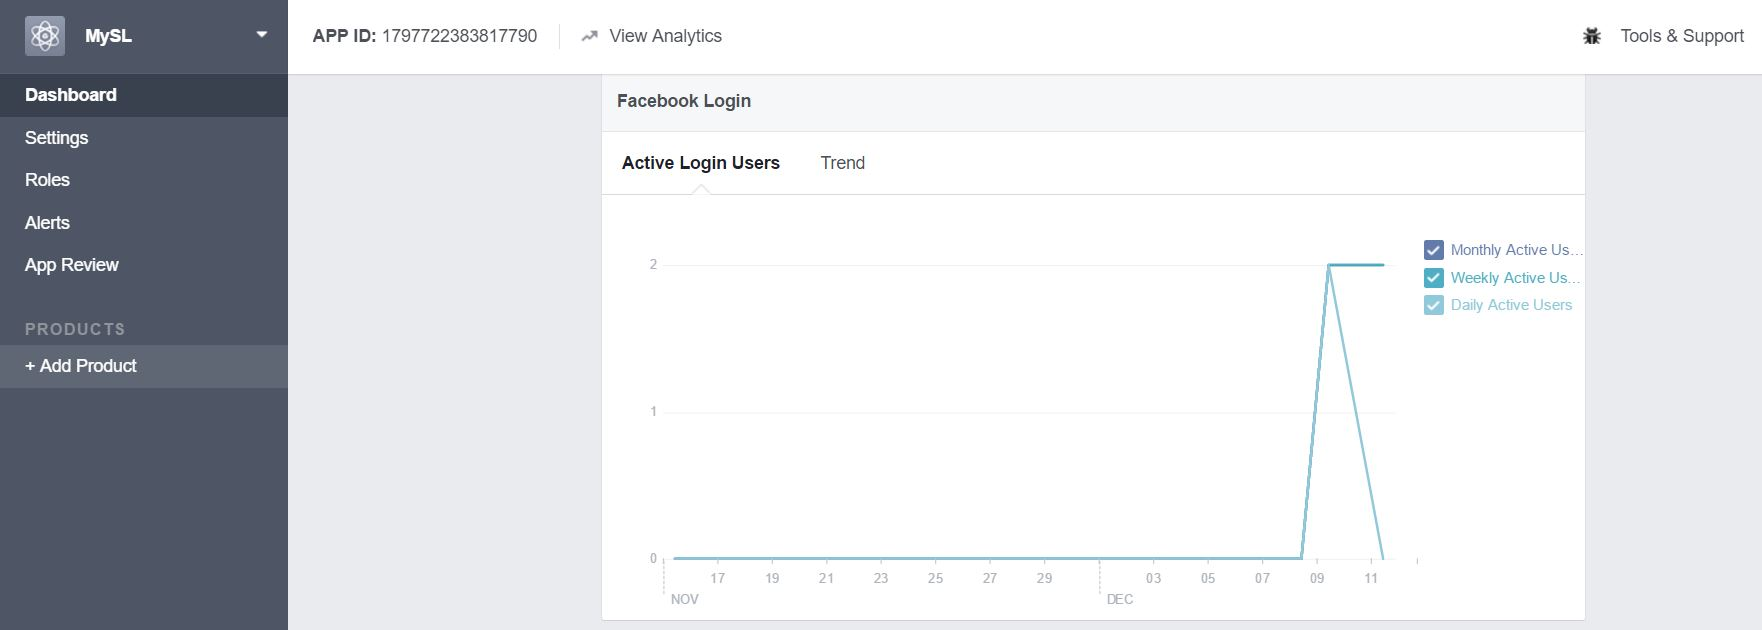
\includegraphics[width=1\textwidth]{jpg/facebook-developers.jpg}
	\caption{Facebook developers dashboard website}
	\label{figure:start-view}
\end{figure}

\begin{figure}
	\centering
	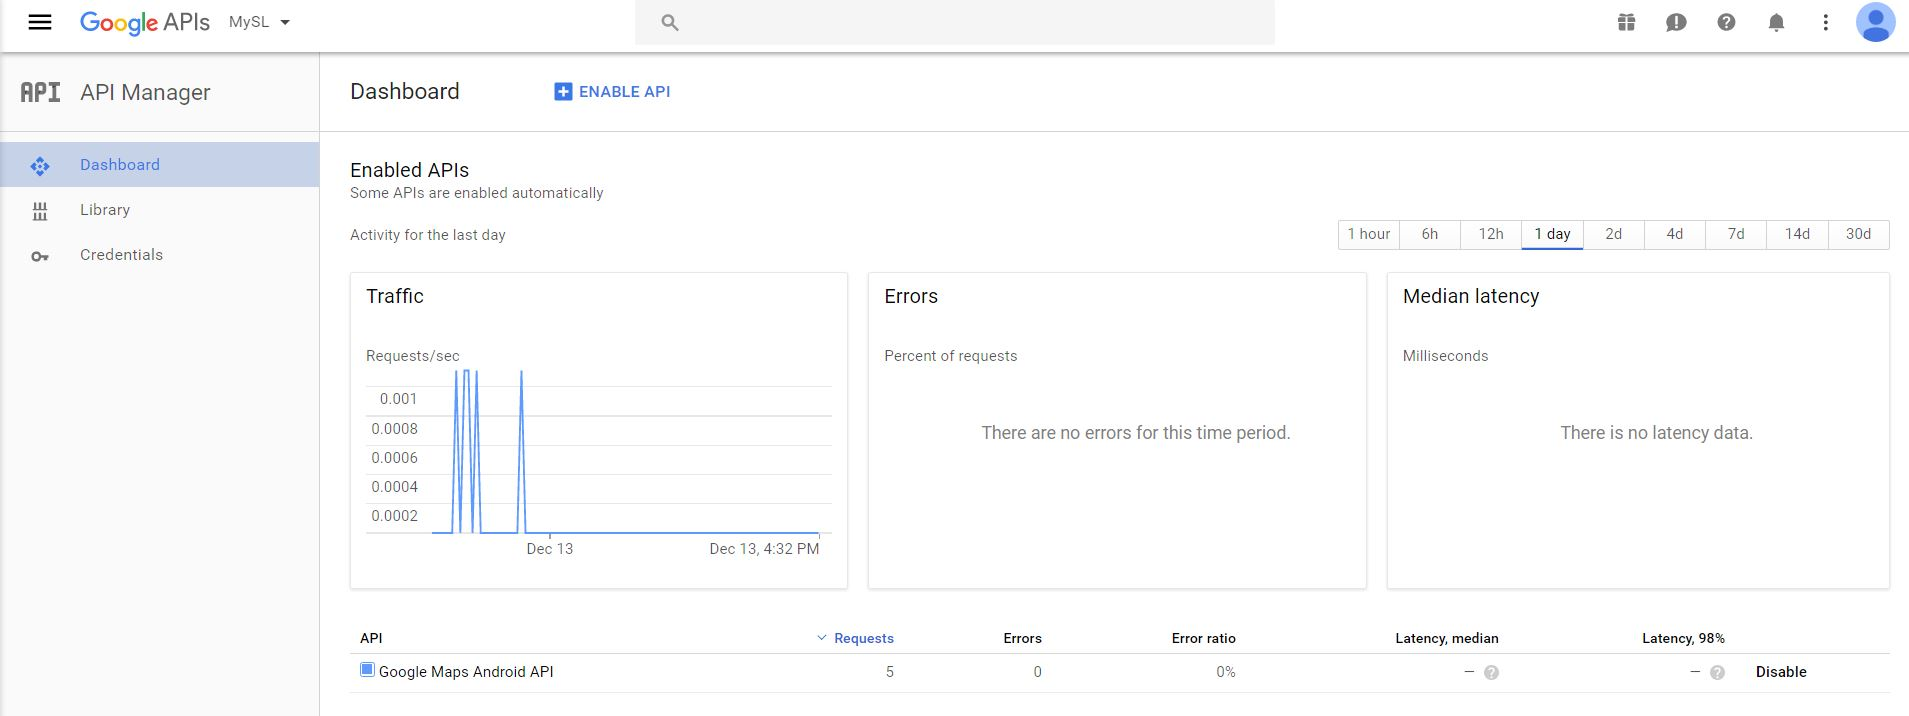
\includegraphics[width=1\textwidth]{jpg/google-developers.jpg}
	\caption{Google developers dashboard website}
	\label{figure:navigation-drawer-in-start-view}
\end{figure}

\begin{figure}
	\centering
	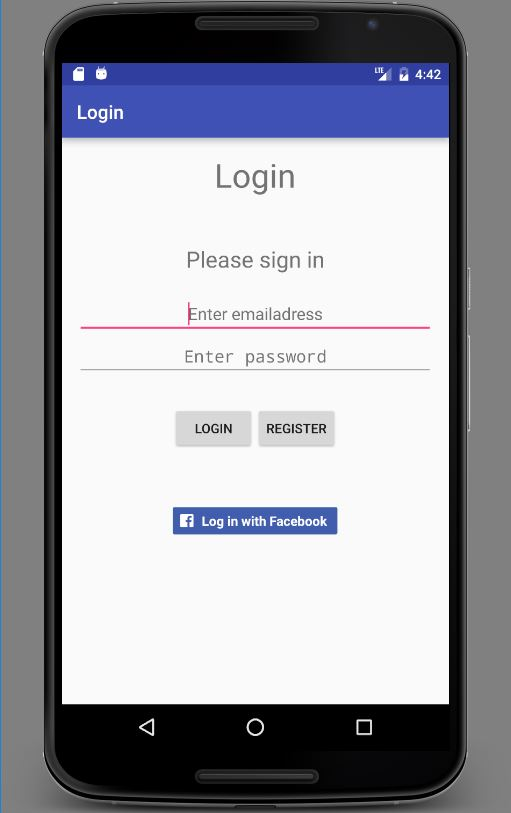
\includegraphics[width=0.4\textwidth]{jpg/facebook1.jpg}
	\caption{Login view with Facebook login button}
	\label{figure:navigation-drawer-in-start-view}
\end{figure}

\begin{figure}
	\centering
	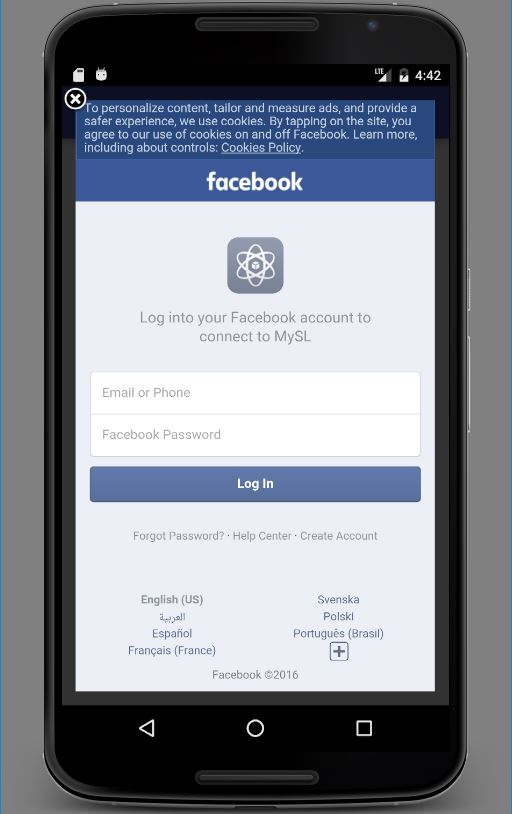
\includegraphics[width=0.4\textwidth]{jpg/facebook2.jpg}
	\caption{Integrated facebook login view}
	\label{figure:search-view}
\end{figure}

\begin{figure}
	\centering
	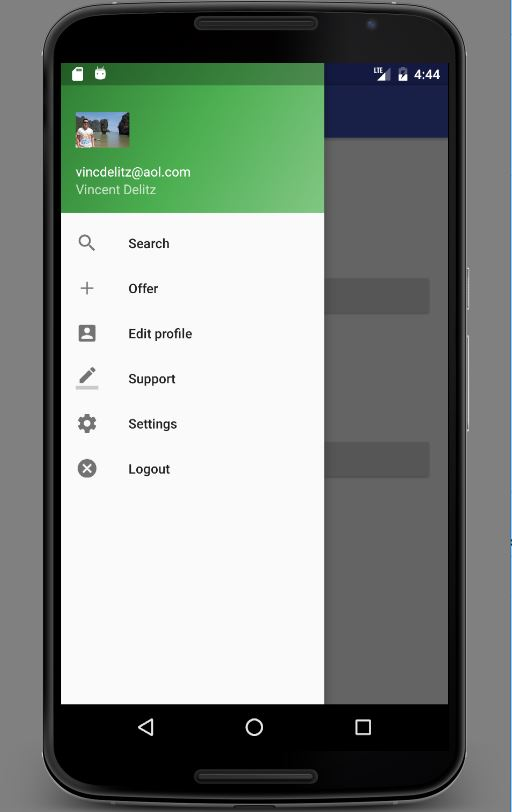
\includegraphics[width=0.4\textwidth]{jpg/facebook3.jpg}
	\caption{Pulled Facebook data and profile picture in the navigation drawer}
	\label{figure:specify-search-view}
\end{figure}

\begin{figure}
	\centering
	\fcolorbox{black}{black}{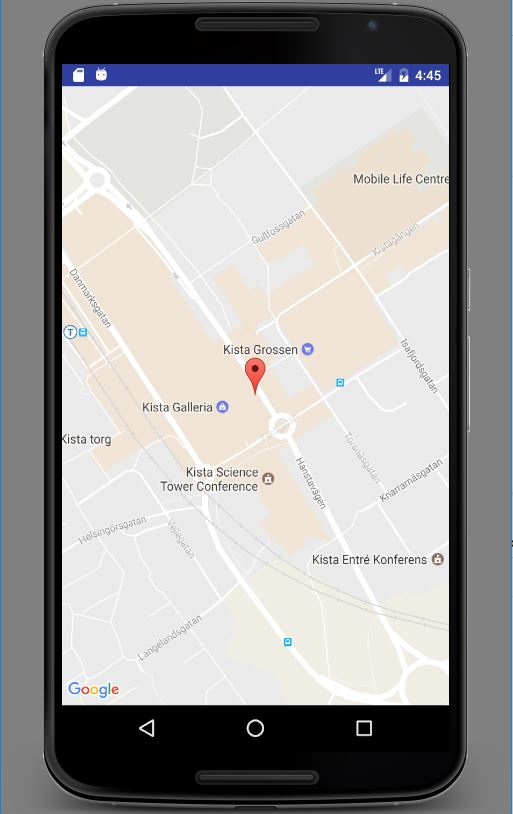
\includegraphics[width=0.4\textwidth]{jpg/google.jpg}}
	\caption{Integrated Google Maps for the pick-up place}
	\label{figure:overview}
\end{figure}

\end{appendices}

\end{document}